

\lstset{ 
    numbers=left, 
    stepnumber=1, 
%    basicstyle=\tiny\ttfamily,
    %basicstyle=\scriptsize\ttfamily,
    basicstyle=\footnotesize\ttfamily,
    captionpos=b, 
    breaklines=true, 
    tabsize=1, 
    numbersep=5pt, 
    xleftmargin=0.5cm,
    keywordstyle=\color{pblue}\bfseries, 
    commentstyle=\color{pgreen}
}

\section{API / Permission-Induced Compatibility Issues}\label{sec-background}

To motivate the research and demonstrate the need for
mechanisms for incompatibility detection, this section
describes three types of Android compatibility issues,
which can lead to runtime app crashes.
Table~\ref{tab:api-mismatch} summarizes API- and
permission-induced compatibility issues.  We will later
show how \@approach helps identify these
incompatibilities.

%\begin{comment}
%In this section, we provide background information related to the Android API and motivate the need for a technique that can effectively identify general API compatibility issues. We also describe and illustrate three types of API and permission-related compatibility issues, summarized in Table \ref{tab:api-mismatch}.
%\end{comment}

\begin{table}[h!]
\centering
\caption{Three Types of Compatibility Issues in Android. \label{tab:api-mismatch}}
%\footnotesize{
%\small{
%\scriptsize{
%\tiny{
\notsotiny{
\begin{tabular*}{\linewidth}{l|c|c|c|c|l}
    \hline
    \hline    
    \multicolumn{1}{c}{}              &\multicolumn{1}{|c}{}    & \multicolumn{1}{|c}{}              & \multicolumn{1}{|c}{App}   & \multicolumn{1}{|c|}{Device}& \\
    \multicolumn{1}{c}{Mismatch type} &\multicolumn{1}{|c}{Abbr.}& \multicolumn{1}{|c}{Compatibility} & \multicolumn{1}{|c}{level} & \multicolumn{1}{|c|}{level} & Results in mismatch if... \\
    \hline \hline
    API invocation                    &API & Backward & \rlap{$\geq\alpha$}\phantom{$<23$} & \rlap{$<\alpha$}\phantom{$\geq23$}    &app invokes API method      \\
    {\it (App $\rightarrow$ Android)} &    & Forward  & \rlap{$<\alpha$}\phantom{$<23$}    & \rlap{$\geq\alpha$}\phantom{$\geq23$} &\mbox{}introduced/updated in $\alpha$ \\
    \hline
    API callback                      &APC & Backward & \rlap{$\geq\alpha$}\phantom{$<23$} & \rlap{$<\alpha$}\phantom{$\geq23$}    &app overrides API callback  \\
    {\it (Android $\rightarrow$ App)} &    & Forward  & \rlap{$<\alpha$}\phantom{$<23$}    & \rlap{$\geq\alpha$}\phantom{$\geq23$} &\mbox{}introduced/updated in $\alpha$ \\
    \hline  
    Permission-                       &PRM & \multirow{ 2}{*}{Forward} & $\geq23$                           & $\geq23$                              &app misuses runtime \\
    induced                            &    &    & $<23$                              & $\geq23$                              &\mbox{}permission checking          \\ 
    \hline
    \hline
\end{tabular*}
}
\end{table}


\subsection{Android API Background}

As of September 2019, there have been 27 releases of the Android API, most recently
API level 29~\cite{android10}.  Each version contains new and
updated methods to help developers improve app performance, security,
and user-experience. In this work, we mainly refer to each release of
the Android API by its API level (e.g., 26) rather than the associated name 
(Oreo) or Android version number (8.0)~\cite{androidversions}. 
Google strongly recommends that developers specify the range of the API levels
their apps can support in the manifest or Gradle file by setting
three attributes: (1) {\tt minSdkVersion}, which specifies the lowest level of the API supported by the app; (2) {\tt targetSdkVersion}, which specifies the level of the API used during app development; and (3) {\tt maxSdkVersion}, which specifies the highest API level supported by the app.\footnote{According to the Google documentation, declaring this attribute is not
    recommended~\cite{sdkversions} but installing an older app on a newer device
    may still lead to unexpected behavior~\cite{Update4}.}

\begin{comment}
\begin{description}[labelindent=2em,leftmargin=!,labelwidth=\widthof{\bfseries The longest label}]
    \item [{\tt minSdkVersion}] The lowest level of the API supported by the app.

    \item [{\tt targetSdkVersion}] The level of the API used during app development.  

    \item [{\tt maxSdkVersion}] The highest level of the
    API supported by the app.\footnote{According to the Google documentation, declaring this attribute is not
    recommended~\cite{sdkversions} but installing an older app on a newer device
    may still lead to unexpected behavior~\cite{Update4}.}

\end{description}
\end{comment}    
    
\subsection{API Compatibility Issues}
\label{API Compatibility Issues}

Incompatible API levels can cause runtime crashes in
Android apps installed on a device running a different
level of the API than that targeted by the app. Changes
to the API are generally additive, so most such crashes
stem from a lack of {\it backward-compatibility}, where
an app targeting a higher API level is installed on a
device running a lower one \cite{sdkversions}. However,
despite Google's assurances, there may also be issues
with {\it forward-compatibility} when an app is run on
a device with a higher API level than the app's target.
If the app invokes a method or overrides a callback
introduced in a newer level of the API than that
supported by the device or removed in a newer level of
the API than targeted by the app, a mismatch arises
(the two red regions as shown in
Figure~\ref{fig:api-mismatch}), which could potentially
crash the app.
%\commentty{Need to clarify the overriding a callback will cause incompatibility, raised by ICSE reviewer1.}

\begin{figure}%{R}{0.5\columnwidth}
    \centering
    %\captionsetup{font=scriptsize,margin=5mm}
    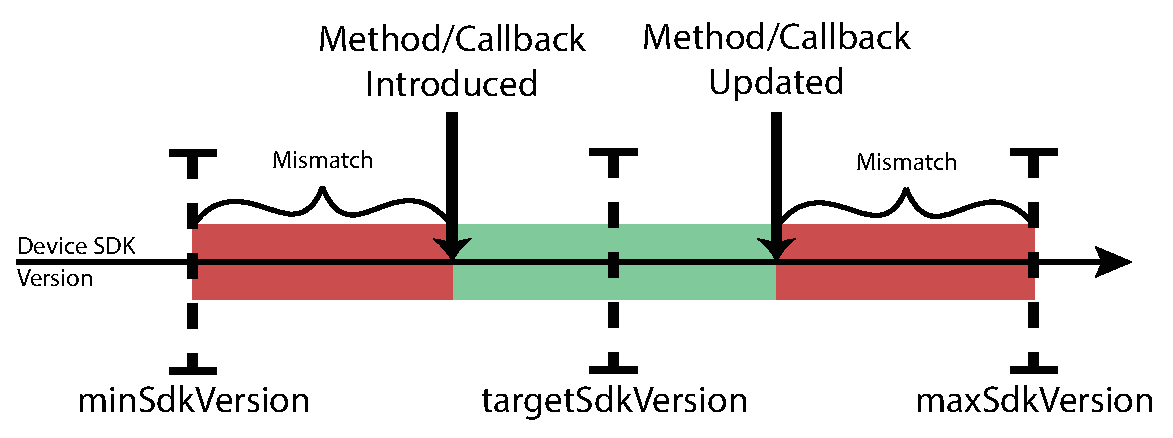
\includegraphics[width=0.85\columnwidth]{images/api-mismatch} 
    \caption{Mismatch between app and device API levels} 
    \label{fig:api-mismatch} 
\end{figure}

We divide these API incompatibilities into two types
(Table~\ref{tab:api-mismatch}): {\it invocation
mismatches}, where an app attempts to invoke an API
method not supported by the device; and {\it callback
mismatches}, where an app implements a callback method
missing from the API level installed on the device,
which will never be invoked.

\subsubsection{API invocation mismatch}

Mismatches in API method invocation occur when an app
developed against a higher version of the API attempts to
call a method introduced between its target version and that
installed on the device; the app crashes when the system
cannot find the desired method. Similarly, an app developed
against a lower version of the API may crash on a device
running a higher version if a method has been removed.
The former is an instance of a backward-compatibility issue, while the latter touches forward-compatibility, as referenced in Table~\ref{tab:api-mismatch}.

\begin{figure}[b]%[8]
%{R}{0.68\columnwidth}
    \lstset{ 
        language=Java, 
        classoffset=1,
        morekeywords={activity_main, text, colorAccent}, 
        keywordstyle=\color{ppurple},
        classoffset=0, 
    } 
    %\captionsetup{font=scriptsize,justification=centering}
    \lstinputlisting[ 
    caption={API Invocation Mismatch}, 
    label={lst:get-color-state-list},
    linebackgroundcolor={ 
        \ifnum \value{lstnumber}=9  \color{highlight} \fi
        \ifnum \value{lstnumber}=10 \color{highlight} \fi 
    } 
    ]{code_snippets/listing1.txt}
\end{figure}

 

Listing~\ref{lst:get-color-state-list} provides an illustrative example, where
the app targets Android API level 28, but its {\tt minSdkVersion} is set to 21.
In case the app is installed on a device with the Android API level 
21---the API level supported by the app according to 
its specified {\tt minSdkVersion}---it will crash on 
the invocation of {\sf getColorStateList}
(lines 9-10), which was introduced in API level 23.
One way to safeguard against this mismatch is to check the device's
API level at runtime, as shown in the comment on line 8.
This prevents the app from executing the call on versions
where it might be missing, but it is not fool-proof;
developers could easily forget to add or modify the check
when updating an app, leaving the code vulnerable to a
mismatch.


\begin{figure}%{R}{0.5\columnwidth} 
    \lstset{language=Java}
    %\captionsetup{font=scriptsize,justification=centering}
    \lstinputlisting[ 
    caption={API Callback Mismatch},
    label={lst:on-attach-context}, 
    linebackgroundcolor={ 
        \ifnum \value{lstnumber}=4 \color{highlight} \fi 
        \ifnum \value{lstnumber}=5 \color{highlight} \fi 
    }
    ]{code_snippets/callback-on-attach.txt} 
\end{figure}


\subsubsection{API callback mismatch}

API callback compatibility issues initiate in the Android system when its invokes callback methods overridden in the app.  Listing \ref{lst:on-attach-context} shows a snippet adapted from the \emph{Simple Solitaire}~\cite{simplesolitaire} app, where the API callback \textsf{onAttach(Context)}, which is introduced in API level 23, is overridden. The app is also specified to run on devices with API level lower than 23, which would not call that method. Thus, any critical actions (e.g., initialization of
an object) performed by the app in that method would be omitted, possibly
leading to runtime crashes. In the case where a callback is added to the API, this mismatch is a backward-compatibility issue; if a callback is removed, it is a problem with forward-compatibility.

\subsection{Permission-induced Compatibility Issues} \label{sec-background:prm}

With the release of Android API level 23 (Android 6), the
Android permission system is completely redesigned.  If a
device is running Android 5.1.1 (API level 22) or below, or
the app's {\tt targetSdkVersion} is 22 or lower, the system
grants all permissions at installation
time~\cite{permissiongroups}. On the other hand, for devices
running Android 6.0 (API level 23) or higher, or when the
app's {\tt targetSdkVersion} is 23 or higher, the app must
ask the user to grant dangerous permissions at runtime.  In
total, Android classifies 26 permissions as
dangerous~\cite{dangerousAPI}.  The goal of the new runtime
permission system is to encourage developers to help users
understand why an application requires the requested
dangerous permission~\cite{runtimepermissions}. 

\begin{figure}[b]%{R}{0.57\columnwidth} 
    \lstset{ 
        language=Java, 
        classoffset=1,
        morekeywords={activity_main, ACTION_IMAGE_CAPTURE},
        keywordstyle=\color{ppurple}, classoffset=0, 
    } 
%    \captionsetup{font=footnotesize}
    \lstinputlisting[
        caption={Permissions Mismatch (tgt $\geq$ 23)}, 
        label={lst:no-runtime-grant}, 
        linebackgroundcolor={ 
            \ifnum \value{lstnumber}=10 \color{highlight} \fi 
            \ifnum \value{lstnumber}=11 \color{highlight} \fi 
            \ifnum \value{lstnumber}=12 \color{highlight} \fi 
        }
    ]{code_snippets/listing3.txt} 
\end{figure}

Permission-induced incompatibility can also be divided into
two types of mismatch: {\it permission request mismatches},
where an app targeting API level 23 or higher does not
implement the new runtime permission checking; and {\it
permission revocation mismatches}, when an app targeting API
22 or earlier runs on a device with API 23 or later and the 
user revokes the use of a dangerous permission used by 
the app at runtime.
 
%\subsubsection{Permission request mismatch}

Listing~\ref{lst:no-runtime-grant} illustrates a permission
request mismatch; the app may crash on line 12 where it
attempts to use a dangerous permission it did not request.
To prevent the mismatch, the app would need to check the API
version and request permissions at runtime (shown as
comments on lines 7-9) and implement {\sf
onRequestPermissionsResult} (line 16). More detailed
examples of the new runtime permissions system can be seen
in the Android documentation \cite{runtimepermissions}.

%\subsubsection{Permission revocation mismatch}

If a user installs an app targeting APIs lower than 23 on a
device running API 23 or above, the user must accept all
dangerous permissions requested by the app at install time,
or the app will not be installed. However, API 23, 
i.e., Android version 6.0, allows the user to revoke those permissions
at any time. If the user revokes any dangerous permission in
the older app's setting after installation, the app would
crash while trying to use that permission--a permissions
revocation mismatch. This behavior has been recurrently
reported in real-world apps. \textit{AdAway}~\cite{adaway},
for example, tries to access external storage (such as an SD
card) at runtime. If that permission is revoked, the app
crashes when its tries to load data from the storage
mechanism.

\subsection{Limitations of Existing Work}
\label{limitations}
One major shortcoming of the state-of-the-art
approaches in detecting API compatibility issues is
their inability to analyze application-under-analysis
and the underlying ADF code in unison.  Existing
analysis techniques first load all code in the project and
then perform analysis on the loaded code.  This
approach is both monolithic and memory intensive.
Moreover, identifying compatibility issues requires analyzing both the application code and ADF in tandem. However, loading both the entire app and the ADF codebase is not feasible, due to high memory consumption. As such, the existing techniques  analyze an app and the underlying ADF separately.
For example, a state-of-the-art technique, called
\textsc{Cider}~\cite{huang2018understanding}, 
conserves memory by creating models from the
underlying ADF to represent API invocations and their callback counterparts. However, as previously reported, constructing ADF models is a daunting and error-prone task that may not be able to keep up with rapid releases of ADFs~\cite{vanderMerwe2012}.
As will be shown in the evaluation section, \textsc{Cider} can miss detecting compatibility issues that exist in different ADFs.
Moreover, it is only capable of detecting compatibility types that have been modeled.

%\textcolor{red}{
Another state-of-the-art incompatibility detector is
\textsc{CiD}\cite{lili2018cid}. This approach creates a
\emph{conditional call graph} for each app to record
method call information along with condition checkers
related to the API level. The construction of this graph is
done by performing an analysis path to identify API
calls. From each API call, \textsc{CiD} performs
backward data-flow analysis to identify the presence of
an API level check. Resolving API usage is then based
on the list of API calls and information from the
\emph{conditional call graph}.  To reduce memory usage,
\textsc{CiD} only analyzes the initial API call and
does not analyze subsequent calls within the
ADF~\cite{lili2018cid}.  As will be shown later, this
approach misses incompatibility issues that exist
deeper into the ADF code.  


Different from all these techniques, our approach
gradually loads classes from both the
application and ADF codebase as needed, and analyzes them all together.  As such, \@approach analysis seamlessly produces a method-call graph that includes methods from both application and ADF classes.  \@approach, therefore, achieves higher effectiveness in detecting different types of API compatibility issues. 

%In the next section, we describe the details of \@approach.  

